%!TEX TS-program = xelatex
\documentclass[]{friggeri-cv}
\usepackage{afterpage}
\usepackage{hyperref}
\usepackage{url}
\usepackage{color}
\usepackage{xcolor}
\hypersetup{
    pdftitle={herve.beraud.cv.en.pdf},
    pdfauthor={herve beraud},
    pdfsubject={Hervé Beraud curriculum vitae},
    pdfkeywords={},
    colorlinks=false,       % no lik border color
   allbordercolors=white    % white border color for all
}
\addbibresource{bibliography.bib}
\RequirePackage{xcolor}
\definecolor{pblue}{HTML}{0395DE}

\begin{document}
\header{Hervé }{Beraud}
    {Full Stack Python Software Engineer}
      
% Fake text to add separator      
\fcolorbox{white}{gray}{\parbox{\dimexpr\textwidth-2\fboxsep-2\fboxrule}{%
.....
}}

% In the aside, each new line forces a line break
\begin{aside}
  \section{Address}
    Rue~Longuebrune~d'astarac
    32450,~Castelnau~Barbarens,~France
    ~
  \section{Contact}
    
\includegraphics[scale=0.50]{img/phone.png}
    +33 661 840 417
    ~
    
\includegraphics[scale=0.50]{img/mail.png}
    \href{mailto:herve.beraud@openmailbox.org}{\textbf{herve.beraud@}\\openmailbox.org}
    ~
  \section{Web \& Git}
    \href{http://www.herve-beraud.ovh}{My Personal Website (click to see)}
    \href{https://github.com/4383}{github.com/4383 (click to see)}
    \href{https://warehouse.python.org/user/4383/}{My Python Account (click to see)}
    ~
  \section{Programming}
    
\includegraphics[scale=0.15]{img/programming.png}
    ~
  \section{OS Preference}
    \textbf{GNU/Linux}
\includegraphics[scale=0.40]{img/5stars.png}
    \textbf{Unix}
\includegraphics[scale=0.40]{img/4stars.png}
    \textbf{MacOS}
\includegraphics[scale=0.40]{img/2stars.png}
    \textbf{Windows}
\includegraphics[scale=0.40]{img/1stars.png}
    ~
  \section{Personal Skills}
    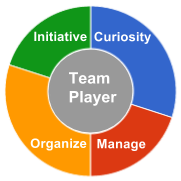
\includegraphics[scale=0.62]{img/personal.png}
    ~
\end{aside}

\section{Personal Philosophy}
    I'm looking for a job where I can really expose my skills and my ideas. I want a job where I'm not only a number. 
    For me quality is greater than benefits.
    The benefits naturally follow quality.
    Not daring to try is the only cardinal sin.

\section{Experience}
\begin{entrylist}
  \entry
    {04-14 - Now}
    {Software Engineer}
    {BULL / EDF, Toulouse, France}
    {Design and develop algorithms, solutions for call center and workload management system. Design and develop multi-channel agent desktop.
    Create and develop Python webapps for generating, deploye, and maintaince version for C\# project (automatized continuouse integration)\\}
  \entry
    {09-13 - 03-14}
    {Embedded Software Engineer}
    {BULL / French Navy, Aix en Provence, France}
    {Design continuous integration, design system architecture , AIX5.3 and Unix software.\\}
    \entry
    {02-13 - 09-13}
    {Software Engineer}
    {BULL / DCNS, Toulon, France}
    {Design and develop electronic warefare system on the FREMM frigate project.\\}
    \entry
    {06-11 - 01-13}
    {Frontend / Backend Web Developer}
    {BULL / Virtual-expo, Marseille, France}
    {Design and development of a world expert online exhibitions website on Linux/Apache/PHP/Zend platform. Design, development of a Python web crawler.\\}
    \entry
    {04-11 - 06-11}
    {System Administrator / Backend Developer}
    {Distrimag, Arles, France}
    {Maintain data center environmental and monitoring equipment (IBM AS400). Virtualize physical server. PHP Development of stock managment software.\\}
    \entry
    {10-10 - 03-11}
    {Frontend Web / Backend Developer}
    {PlusValue SAS, Vitrolles, France}
    {Management and migration of servers. Development of php web micro-framework. Development of web templates and interfaces. Management of SQL databases.\\}
    \entry
    {12-04 - 01-09}
    {Buisness Owner}
    {Damofli Fruits \& Legumes, France}
    {Manage marketing operations, accounting, sales plans, inventory management.\\}
    \entry
    {09-01 - 11-04}
    {Landscape Architect}
    {Local Council of Martigues, France}
    {Manage marketing operations, accounting, sales plans, inventory management.}
\end{entrylist}

\newpage
\section{Education}
\begin{entrylist}
  \entry
    {2010 - Now}
    {Master's Degree in Computer Engineering}
    {CNAM Aix en Provence, France}
    {Curriculum information systems.\\
    Main subjects: Systems \& Software Architecture and Security, Urbanism for Evolving Systems.\\}
  \entry
    {2009 - 2010}
    {BTEC Higher National Diploma in Software Development}
    {AFPA Istres, France}
    {Main subjects: Software Architecture, Modeling Tools (Merise, UML).\\}
  \entry
    {1999 - 2001}
    {BTEC National Diploma in Landscape Architect}
    {Lycée Fontlongue Miramas, France}
    {Agricultural college.\\
    Main subjects: Design and Advise on the Construction of Urban, Rural, Residential and Public Landscape.\\}
  \entry
    {1999 - 2001}
    {BTEC First Diploma in Nursery Gardener}
    {Lycée Fontlongue Miramas, France}
    {Agricultural college.\\
    Main subjects: Cultivating, Harvesting, Transplanting Trees, Shrubs or Plants.}
\end{entrylist}

\section{Significative Realisations and Personal projects}
\begin{entrylist}
  \entry
    {10-2015}
    {\href{http://pypi.python.org/pypi/barcode-generator/0.1rc15}{Barcode Generator (click to see)}}
    {Personal project}
    {\emph{Python 3 / SVG / Git}}
  \entry
    {07-2015}
    {\href{http://www.the-street-workout-database.ovh}{The Street Workout Database (click to see)}}
    {Personal project}
    {\emph{Python / Django / Debian 7 / PostGreSQL / Nginx / Supervisor / Git}}
  \entry
    {12-2014}
    {\href{http:www.herve-beraud.ovh}{My personal website (click to see)}}
    {Personal project}
    {\emph{Python / Django / Debian 7 / PostGreSQL / Nginx / Supervisor / Git}}
  \entry
    {02-2013}
    {\href{https://github.com/4383/fabric-debian/}{Security Best Practices Automatic Setup (click to see)}}
    {Personal project}
    {\emph{Python / Iptables /  debian 6 / port-knocking / Fail2Ban / PostGreSQL / Nginx}}
  \entry
    {2012}
    {\href{http://medical-expo.com}{Medical Expo (click to see)}}
    {Professional project}
    {\emph{PHP5.3 / Apache 2 / Mysql 5}}
  \entry
    {10-2012}
    {\href{http://github.com/4383/battle-story/}{Battle-Story Video Game (click to see)}}
    {Personal project}
    {\emph{Python / Pygame}}
  \entry
    {09-2012}
    {\href{http://github.com/4383/WebForge/}{HTTP request forgery (click to see)}}
    {Personal project}
    {\emph{Python / Tkinter}}
  \entry
    {2010}
    {\href{http://fr.wikipedia.org/wiki/Neo\_Keyboard}{Neo Keyboard - Virtual Piano (click to see)}}
    {Personal project}
    {\emph{C / C++ / SDL}}
  \entry
    {2010}
    {\href{http://fr.wikipedia.org/wiki/Metronomix}{Metronomix - Virtual Metronome (click to see)}}
    {Personal project}
    {\emph{C / C++ / SDL}}
\end{entrylist}


\begin{aside}
~
~
~
  \section{I Like It}
    
\includegraphics[scale=0.18]{img/python.png}
    
\includegraphics[scale=0.18]{img/arch.png}
    
\includegraphics[scale=0.06]{img/vim.png}
    
\includegraphics[scale=0.06]{img/latex.png}
    
\includegraphics[scale=0.08]{img/gnu.png}
    \href{http://www.herve-beraud.ovh/skills/}{And More...}
    ~
  \section{About me}
    Year of birth : 1982
    married, 4 childrens 
    ~
  \section{Languages}
    \textbf{French}
\includegraphics[scale=0.40]{img/5stars.png}
    \textbf{English}
\includegraphics[scale=0.40]{img/3stars.png}
\end{aside}

\section{Hobbies and Interests}
\begin {itemize}
    \item \emph {Sports (Street Workout, Swimming, Running)}
    \item \emph {Family}
    \item \emph {Computer Sciences (ArchLinux, Python, Arduino, Vim)}
    \item \emph {Psychology / Philosophy}
    \item \emph {Traveling (Senegal, Ivory Coast, Europe)}
\end {itemize}
\begin{flushright}
\emph{Latest update - December, 2015}
\end{flushright}
\end{document}
